

\subsubsection{Vektoren und Matrizen}
\small

\begin{concept}{Vektoren Eigenschaften und Formeln}
    \begin{itemize}
        \item Länge/Betrag: $\abs{\vec{a}}=\sqrt{a_1^2+a_2^2+\cdots+a_n^2}$
        \item Einheitsvektor/Normierung: $\vec{e_a}=\frac{1}{a}\cdot\vec{a} = \frac{\overrightarrow{a}}{|\overrightarrow{a}|}$
        \item Orthogonal (Senkrecht): $\overrightarrow{a} \cdot \overrightarrow{b} = 0 \rightarrow \text{ orthogonal}$ (90° Winkel)
        \item Vektoraddition: $\begin{psmallmatrix} a_x + b_x\\ a_y + b_y \end{psmallmatrix}$ und Skalarmultiplikation: $\begin{psmallmatrix} \lambda \cdot a_x \\ \lambda \cdot a_y \end{psmallmatrix}$
        \item Skalarprodukt: $\overrightarrow{a} \cdot \overrightarrow{b} = a_x \cdot b_x + a_y \cdot b_y = |\overrightarrow{a}| \cdot |\overrightarrow{b}| \cdot \cos(\varphi)$
        \item Kreuzprodukt: $\overrightarrow{a} \times \overrightarrow{b}$ ist orthogonal zu $\overrightarrow{a}$ und $\overrightarrow{b}$\\
        $\overrightarrow{a} \times \overrightarrow{b} = \begin{psmallmatrix}{ccc}
            a_y \cdot b_z &-& a_z \cdot b_y \\
            a_z \cdot b_x &-& a_x \cdot b_z \\
            a_x \cdot b_y &-& a_y \cdot b_x
            \end{psmallmatrix}$
    \end{itemize}
\end{concept}


\raggedcolumns

    \begin{definition}{Matrix}
        Tabelle mit $m$ Zeilen und $n$ Spalten: $m \times n$-Matrix $A$\\
        $a_{ij}$: Element in der $i$-ten Zeile und $j$-ten Spalte
    \end{definition}
    

    \begin{formula}{Addition und Subtraktion}
        $A + B = C \rightarrow c_{ij} = a_{ij} + b_{ij}$
    \end{formula}

    \begin{formula}{Skalarmultiplikation}
        $k \cdot A = B \rightarrow b_{ij} = k \cdot a_{ij}$
    \end{formula}



    \begin{formula}{Matrixmultiplikation} $A^{m \times n}$, $B^{n \times k}$\\
        \begin{minipage}{0.6\linewidth}
        Bedingung: $A$ $n$ Spalten, $B$ $n$ Zeilen.\\
        Resultat: $C$ hat $m$ Zeilen und $k$ Spalten.
        \begin{itemize}
            \item $A \cdot B = C$
            \item $c_{ij} = a_{i1} \cdot b_{1j} + a_{i2} \cdot b_{2j} + \ldots + a_{in} \cdot b_{nj}$
            \item $A \cdot B \neq B \cdot A$
        \end{itemize}  
        \end{minipage}
        \begin{minipage}{0.35\linewidth} 
        \vspace{-5mm}
        \begin{center}
        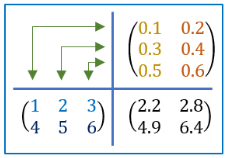
\includegraphics[width=0.8\linewidth]{matrixmultiplikation.png}
        \end{center}
        \end{minipage}
    \end{formula}


    \begin{minipage}{0.65\linewidth}
        \begin{definition}{Transponierte Matrix} $A^{m \times n} \rightarrow (A^T)^{n \times m}$
            \begin{itemize}
                \item $A^T$: Spalten und Zeilen vertauscht
                \item $(A^T)_{ij} = A_{ji}$ und ${(A\cdot B)}^T = B^T\cdot A^T$
            \end{itemize}
        \end{definition}
    \end{minipage}
    \begin{minipage}{0.35\linewidth}
        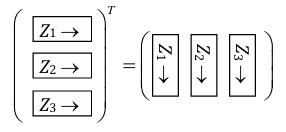
\includegraphics[width=1\linewidth]{mat-transpos.png}
    \end{minipage}

    \begin{KR}{Spezielle Matrizen}
        \begin{itemize}
            \item \textbf{Symmetrische Matrix}: $A^T = A$
            \item \textbf{Einheitsmatrix}: $E$ mit $e_{ij} = 1$ für $i = j$ und $e_{ij} = 0$ für $i \neq j$
            \item \textbf{Diagonalmatrix}: $a_{ij} = 0$ für $i \neq j$
            \item \textbf{Dreiecksmatrix}: $a_{ij} = 0$ für $i > j$ (obere Dreiecksmatrix) \\oder $i < j$ (untere Dreiecksmatrix)
        \end{itemize}
    \end{KR}

  
\begin{concept}{Permutationsmatrix} $P$ ist eine Matrix, die aus der Einheitsmatrix durch Zeilenvertauschungen entsteht. 
    \vspace{1mm}\\
    \begin{minipage}[t]{0.5\textwidth}
        Für die Vertauschung der $i$-ten und $j$-ten Zeile hat $P_k$ die \textbf{Form}:
        \begin{itemize}
            \item $p_{ii} = p_{jj} = 0$ 
            \item $p_{ij} = p_{ji} = 1$
            \item Sonst gleich wie in $E_n$
        \end{itemize}
    \end{minipage}
    \hspace{3mm}
    \begin{minipage}[t]{0.45\textwidth}
        \vspace{1mm}
        \textbf{Wichtige Eigenschaften}:
        \begin{itemize}
            \item $P^{-1} = P^T = P$
            \item Mehrere Vertauschungen:\\ $P = P_l \cdot ... \cdot P_1$
        \end{itemize}
    \end{minipage}
\end{concept}

\subsubsection{Quadratische Matrizen}
  
    \begin{theorem}{Eigenschaften invertierbarer Matrizen}
        \begin{itemize}
            \item $A\cdot A^{-1}=A^{-1}\cdot A=E$ und $(A^{-1})^{-1}=A$
            \item ${(A\cdot B)}^{-1}=B^{-1}\cdot A^{-1}$ {\small $\quad$ Die Reihenfolge ist relevant!}
            \item $A$ und $B$ invertierbar $\Rightarrow$ $AB$ invertierbar
            \item ${(A^T)^{-1}}={(A^{-1})}^T$ $\quad$ $A$ invertierbar $\Rightarrow$ $A^T$ invertierbar
        \end{itemize}
    \end{theorem}

\begin{theorem}{Inverse einer $2 \times 2$-Matrix} $A = \begin{psmallmatrix} a & b \\ c & d \end{psmallmatrix}$ mit $det(A) = ad - bc$\\
        $A^{-1} = \frac{1}{\det(A)} \cdot \begin{pmatrix} d & -b \\ -c & a \end{pmatrix}$
        $\rightarrow$ NUR Invertierbar falls $ad - bc \neq 0$
\end{theorem}

\begin{KR}{Inverse berechnen} einer quadratischen Matrix $A^{n \times n}$
    $$A \cdot A^{-1} = E \rightarrow ( A | E ) \leadsto \text{Zeilenoperationen} \leadsto ( E | A^{-1})$$
\end{KR}

\raggedcolumns
\columnbreak

\subsubsection*{Lineare Gleichungssysteme (LGS)}
    
        \begin{definition}{Lineares Gleichungssystem (LGS)}
            
            Matrixform $A\cdot\vec{x}=\vec{b}$:

            
            \begin{minipage}{0.55\linewidth}
                $\begin{psmallmatrix} a_{11} & \cdots & a_{1n} \\ \scalebox{0.5}{\vdots} & \cdots & \scalebox{0.5}{\vdots} \\ a_{m1} & \cdots & a_{mn} \end{psmallmatrix} \cdot \begin{psmallmatrix}
                    x_1 \\ \scalebox{0.5}{\vdots} \\ x_n
                \end{psmallmatrix} = \begin{psmallmatrix}
                    b_1 \\ \scalebox{0.5}{\vdots} \\ b_m
                \end{psmallmatrix}$
            \end{minipage}
            \begin{minipage}
                {0.45\linewidth}
                {\small
                $A$: Koeffizientenmatrix\\
                $\vec{x}$: Vektor der Unbekannten\\
                $\vec{b}$: Vektor der Konstanten}
            \end{minipage}
        \end{definition}

    
        \begin{theorem}{Rang einer Matrix} $rg(A)$ = Anzahl Zeilen - Anzahl Nullzeilen
            
            $\Rightarrow$ Anzahl linear unabhängiger Zeilen- oder Spaltenvektoren
        \end{theorem}


\begin{concept}{Zeilenstufenform (Gaussii)}
    \begin{itemize}
        \item Alle Nullen stehen unterhalb der Diagonalen, Nullzeilen zuunterst
        \item Die erste Zahl $\neq 0$ in jeder Zeile ist eine führende Eins
        \item Führende Einsen, die weiter unten stehen $\rightarrow$ stehen weiter rechts
    \end{itemize}
\end{concept}

\begin{KR}{Zeilenperationen} erlaubt bei LGS (z.B. Gauss-Verfahren)
        \begin{itemize}
            \item Vertauschen von Zeilen
            \item Multiplikation einer Zeile mit einem Skalar
            \item Addition eines Vielfachen einer Zeile zu einer anderen
        \end{itemize}
    \end{KR}
    
    

    

    \begin{theorem}{Lösbarkeit von linearen Gleichungssystemen}

        \begin{minipage}{0.5\linewidth}
            \begin{itemize}
                \item Lösbar: $rg(A) = rg(A|b)$
                \item genau eine Lösung: $rg(A) = n$
            \end{itemize}
        \end{minipage}
        \begin{minipage}{0.5\linewidth}
            \begin{itemize}
                \item unendlich viele Lösungen:\\ $rg(A) < n$
            \end{itemize}
        \end{minipage}
    \end{theorem}

    \begin{KR}{Parameterdarstellung} bei unendlich vielen Lösungen

        \begin{minipage}{0.74\linewidth}
            Führende Unbekannte: Spalte mit führender Eins\\
            Freie Unbekannte: Spalten ohne führende Eins
        \end{minipage}
        \begin{minipage}{0.25\linewidth}
            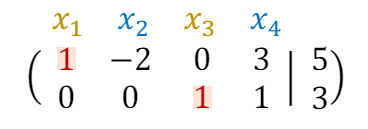
\includegraphics[width=1\linewidth]{parameterdarstellung_lgs.png}
        \end{minipage}
    \end{KR}

    \begin{definition}{Homogenes LGS}
        $\vec{b}=\vec{0} \rightarrow A\cdot\vec{x}=\vec{0} \rightarrow rg(A)=rg(A\mid\vec{b})$
            \begin{itemize}
                \item eine Lösung $x_1=x_2=\cdots=x_n=0$, die sog. \textit{triviale Lösung}.
                \item unendlich viele Lösungen
            \end{itemize}
    \end{definition}

    \begin{theorem}{Koeffizientenmatrix{,} Determinante{,} Lösbarkeit des LGS }\\
        Für $n\times n$-Matrix $A$ sind folgende Aussagen äquivalent:
    
        \vspace{1mm}
    
        \begin{minipage}{0.3\linewidth}
            \begin{itemize}
                \item $\det(A)\neq 0$
                \item $rg(A)=n$
                \item $A$ ist invertierbar
            \end{itemize}
        \end{minipage}
        \begin{minipage}{0.7\linewidth}
            \begin{itemize}
                \item Spalten von $A$ sind linear unabhängig.
                \item Zeilen von $A$ sind linear unabhängig.
                \item LGS $A\cdot\vec{x}=\vec{0}$ \\hat eindeutige Lösung $x=A^{-1}\cdot 0=0$
            \end{itemize}
        \end{minipage}
    \end{theorem}

    




\subsubsection{Fehleranalyse}

\begin{concept}{Wichtige Normen}

\textbf{1-Norm:}
        $\|x\|_1 = \sum_{i=1}^n |x_i|,
        \|A\|_1 = \max_j \sum_{i=1}^n |a_{ij}|$

\textbf{2-Norm:}
        $\|x\|_2 = \sqrt{\sum_{i=1}^n x_i^2}, 
        \|A\|_2 = \sqrt{\rho(A^TA)}$

$\infty$\textbf{-Norm:}
        $\|x\|_\infty = \max_i |x_i|, 
        \|A\|_\infty = \max_i \sum_{j=1}^n |a_{ij}|$
\end{concept}

\begin{theorem}{Fehlerabschätzung für LGS}\\
Sei $\|\cdot\|$ eine Norm, $A \in \mathbb{R}^{n\times n}$ regulär und $Ax = b$, $A\tilde{x} = \tilde{b}$
\vspace{1mm}\\
\begin{minipage}[t]{0.47\textwidth}
    \textbf{Absoluter Fehler:}
    \vspace{-5mm}\\
    \begin{center}
        $\|x - \tilde{x}\| \leq \|A^{-1}\| \cdot \|b - \tilde{b}\|$
    \end{center}
\end{minipage}
\hspace{2mm}
\begin{minipage}[t]{0.47\textwidth}
    \textbf{Relativer Fehler:}
    \vspace{-5mm}\\
    \begin{center}
        $\frac{\|x - \tilde{x}\|}{\|x\|} \leq \text{cond}(A) \cdot \frac{\|b - \tilde{b}\|}{\|b\|}$
    \end{center}
\end{minipage}
\vspace{1mm}\\
Mit der Konditionszahl $\text{cond}(A) = \|A\| \cdot \|A^{-1}\|$
\end{theorem}

\begin{concept}{Konditionierung}\\
Die Konditionszahl beschreibt die numerische Stabilität eines LGS:
\begin{itemize}
    \item $\text{cond}(A) \approx 1$: gut konditioniert
    \item $\text{cond}(A) \gg 1$: schlecht konditioniert
    \item $\text{cond}(A) \to \infty$: singulär
\end{itemize}
\end{concept}



\raggedcolumns
\columnbreak

\subsubsection{Determinante}

    \begin{definition}{Determinante} $det(A) \neq 0 \rightarrow A$ ist invertierbar
    \end{definition}

    

    \begin{definition}{Geometrische Interpretation} der Determinante:\\
        Fläche im $\mathbb{R}^2$ und Volumen im $\mathbb{R}^3$
        durch eine Matrix A aufgespannt:
        $A = |\vec{a} \times \vec{b}| = |\det(A)|$
    \end{definition}

   
    
    \begin{theorem}{Eigenschaften von Determinanten}{\footnotesize mit $A, B \in \mathbb{R}^{n \times n}$, $\lambda \in \mathbb{R}$}\\
        \begin{minipage}{0.5\linewidth}
            \begin{itemize}
                \item $\det(A \cdot B) = \det(A) \cdot \det(B)$
                \item $\det(\lambda \cdot A) = \lambda^n \cdot \det(A)$
                \item $\det(A) = 0 \Leftrightarrow A$ ist singulär
                
            \end{itemize}
        \end{minipage}
        \begin{minipage}{0.5\linewidth}
            \begin{itemize}
                \item $\det(E) = 1$
                \item $\det(A^T) = \det(A)$
                \vspace{1mm}
                \item $\det(A^{-1}) = \frac{1}{\det(A)}$
            \end{itemize}
        \end{minipage}

        \vspace{1mm}

        {\footnotesize $E$ = Einheitsmatrix}
    \end{theorem}

    \begin{formula}{Determinante $1\times 1$-Matrix} $\det(A)=A_{11}$
    \end{formula}
    
    \begin{formula}{Determinante $2 \times 2$-Matrix}
        $A = \begin{psmallmatrix} a & b \\ c & d \end{psmallmatrix}$
        $\det(A) = |A| = a \cdot d - b \cdot c$
    \end{formula}

    \begin{minipage}{0.7\linewidth}
    \begin{formula}{Determinante $3 \times 3$-Matrix}
        $A = \begin{psmallmatrix} a & b & c \\ d & e & f \\ g & h & i \end{psmallmatrix}$

        $|A| = a \cdot e \cdot i + b \cdot f \cdot g + c \cdot d \cdot h - c \cdot e \cdot g - b \cdot d \cdot i - a \cdot f \cdot h$
    \end{formula}
    \end{minipage}
    \begin{minipage}{0.3\linewidth}
        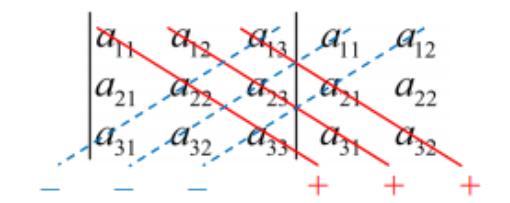
\includegraphics[width=1\linewidth]{determinante_3x3.png}
    \end{minipage}
    
    \begin{concept}{Determinante $n \times n$-Matrix}\\
        $\det(A) = |A| = \sum_{i=1 \text{ oder } j=1}^{n} (-1)^{i+j} \cdot a_{ij} \cdot |A_{ij}|$

        \textcolor{pink}{Tipp:} Entwickeln nach Spalte oder Zeile mit den meisten Nullen!
    \end{concept}

    \begin{KR}{Tricks und Tipps}
        \begin{itemize}
            \item hat $A$ eine Nullzeile oder -spalte, so ist $\det(A) = 0$
            \item hat $A$ zwei gleiche Zeilen oder Spalten, so ist $\det(A) = 0$
            \item $\det(A) \neq 0$ $\Rightarrow$ Spalten/Zeilen sind linear unabhängig
        \end{itemize}
    \end{KR}

    \begin{formula}{Determinante mit Gauss} Spezialfall \textcolor{pink}{Dreiecks- /Diagonalmatrix}

        Wende Gauss-Algorithmus an, um $A$ in Dreiecksform zu bringen.\\ Es gilt für jede Dreiecksmatrix oder Diagonalmatrix $D$:\\
        $\det(D) = (-1)^k \prod_{i=1}^n d_{ii}$

        {\small $k$ = Anzahl der Zeilen-Vertauschungen}\\
        {\small Bei Skalarmultiplikationen ändert sich $\det(A)$ um den Skalierungsfaktor}
    \end{formula}

\subsubsection{Matrix-Zerlegungen}

\begin{KR}{LR-Zerlegung}
    $(E | A | E) \underbrace{\leadsto}_{Gauss} (P | R | L)$
    
    Vorwärtseinsetzen: $Ly = b$
    Rückwärtseinsetzen: $Rx = y$
\end{KR}

\begin{KR}{QR-Zerlegung} (noch genauer erklären)
    \begin{itemize}
        \item $A = Q \cdot R$ mit $Q$ orthogonal und $R$ obere Dreiecksmatrix
        \item $Q^T = Q^{-1}$
        \item $R$ ist eindeutig, $Q$ nicht
    \end{itemize}
\end{KR}

































